\documentclass[tikz]{standalone}
\begin{document}

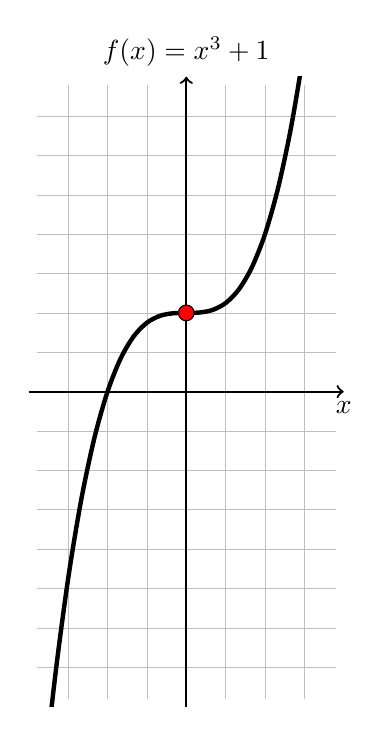
\begin{tikzpicture}[scale=1]
  \draw[very thin,color=lightgray,step=0.5] (-1.9,-3.9) grid (1.9,3.9);
  \draw[->,thick] (-2,0) -- (2,0) node[below] {$x$}; 
  \draw[->,thick] (0,-4) -- (0,4) node[above] {$f(x)=x^3+1$};
  \clip (-2,-4) rectangle (2,4);
  \draw[ultra thick,smooth,domain=-2:2]	plot (\x,\x*\x*\x+1) ;
  %\node[below right] at (2,8) {$f(x) = x^3$};
  \draw[fill = red] (0,1) circle [radius = .1];
  %\node[align=center,below right] at (0,0) {Not a relative\\extrema};
\end{tikzpicture}
\hspace{1cm}
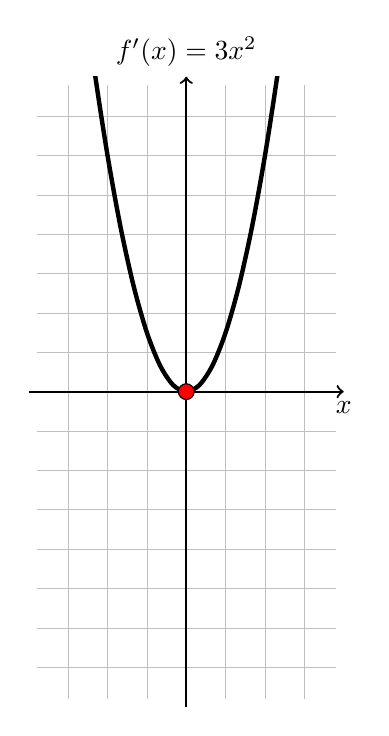
\begin{tikzpicture}[scale=1]
  \draw[very thin,color=lightgray,step=0.5] (-1.9,-3.9) grid (1.9,3.9);
  \draw[->,thick] (-2,0) -- (2,0) node[below] {$x$}; 
  \draw[->,thick] (0,-4) -- (0,4) node[above] {$f'(x)=3x^2$};
  \clip (-2,-4) rectangle (2,4);
  \draw[ultra thick,smooth,domain=-2:2]	plot (\x,3*\x*\x) ;
  %\node[below right] at (2,8) {$f(x) = x^3$};
  \draw[fill = red] (0,0) circle [radius = .1];
  %\node[align=center,below right] at (0,0) {Not a relative\\extrema};
\end{tikzpicture}
\end{document} 
